\appendix

\section{Additional Details}
\label{app:details}

\paragraph{Metrics.}
We evaluate GSM8K with two accuracy numbers and two cost numbers.
Any-finished $\uparrow$ is the fraction of problems for which any admitted residual produces the reference number.
Winner $\uparrow$ is the fraction for which the residual selected as the winner does.
Prefill $\downarrow$ is the measured GPU prefill token total.
Time $\downarrow$ is end-to-end wall-clock seconds on four A100 40GB GPUs.
For MATH-500 we report any-finished and time on the first $32$ problems at level $4$ or higher.
Peak KV is the maximum live bytes of key--value cache; offered load is the concurrent request rate under a $1$\,s P99 time-to-first-token line.

\paragraph{Hosts.}
ESC uses an agreement window of length $5$.
On the controlled mix the window does not fill, so an admitted residual runs to $D{=}512$.
Speculative rejection uses horizon $256$ and dropped fraction $0.5$, applied to the admitted set.
DPTS uses a mini-step of $100$ tokens.
The memory-limit early trigger from speculative rejection does not activate at $k \le 16$ on this hardware.

\paragraph{Admission rules.}
The default rule keeps every residual at or above $\tau_{\mathrm{pre}}$, including index $0$.
Winner-only keeps a single reserved slot and ignores the score.
Both are measured at a fixed batch width in Table~\ref{tab:best}.
\sys is implemented on top of the host-alone baseline.
It is complementary to the hosts, since it does not modify their scoring rules.

\paragraph{Controlled mix.}
For each problem, half of the residuals are live strategy instructions and half alternate a repeated loop with illegal text.
Index $0$ is always live.
The mix is a controlled test of the two bars, not a production trace.
Worked strings are in Appendix~\ref{app:examples}.

\section{Score Functions}
\label{app:scores}

The runs in this paper use one ordered pair,
\begin{equation}
\label{eq:pair}
(\tau_{\mathrm{pre}}, \tau_{\mathrm{dec}}) = (0.15,\ 0.45).
\end{equation}
A loop scores $0.02$ on the residual and $0.04$ on a prefix.
Illegal text scores $0.22$ on the residual and $0.16$ on a prefix.
An answer mark scores $0.92$.
Thus $\tau_{\mathrm{pre}}$ sits between a loop and illegal text, and $\tau_{\mathrm{dec}}$ sits between an illegal prefix and an answer mark.
Raising the prefill bar to $\tau_{\mathrm{dec}}$ is the faster operating point reported in the tables.

Both scorers are deterministic functions of a string.
They do not call the model.
Table~\ref{tab:score-examples} evaluates the residual kinds in the controlled mix.

\begin{table}[h]
\centering
\small
\setlength{\tabcolsep}{4pt}
\begin{tabular}{@{}p{0.42\columnwidth}lcc@{}}
\toprule
Text & Reason & Prefill & Decode \\
\midrule
Repeated \texttt{*loop*} span & loop & 0.02 & 0.04 \\
\texttt{undefined nan \ldots} & illegal & 0.22 & 0.16 \\
Live strategy instruction & ok & $\approx 1.00$ & --- \\
Prefix containing \texttt{\#\#\#\#} or \texttt{\textbackslash boxed} & answer & --- & 0.92 \\
Empty string & empty & 0.00 & 0.00 \\
\bottomrule
\end{tabular}
\caption{Scores on the residual kinds in the evaluation mix.
A dash means that scorer is not applied to that string.
The decode column is the score of a generated prefix of that kind, not a second pass over the residual.}
\label{tab:score-examples}
\end{table}

\paragraph{Prefill.}
After the loop and illegal tests, \eqref{eq:prefill-score} mixes an alphanumeric fraction with character uniqueness.
The coefficients $0.55$ and $0.45$ are fixed.
The measurements score the residual text.

\paragraph{Decode.}
The answer-mark test runs before the illegal test, so a prefix that both looks noisy and contains an answer mark is an answer ($0.92$).
The numeric mix in \eqref{eq:decode-score} adds digit and operator mass so that a healthy math prefix can continue before an answer mark appears.
The planner prior that decides who is probed is
\[
0.35\,\min(1,2\alpha) + 0.65\,\min(1,8\eta)
\]
on the residual, with loop $0.04$ and illegal $0.16$.
It ranks residuals for the host.
It is not substituted for $s^{\mathrm{pre}}$.

\paragraph{Early prefix inside prefill.}
A separate test, not used by the tables in Section~\ref{sec:eval}, inspects the first fraction $\alpha{=}0.20$ of a residual.
It fires when that slice scores below $\tau_{\mathrm{pre}}$ for a reason other than ordinary text.
The reported measurements use the full-residual loop test rather than this partial abort.

\section{Proof of Proposition~\ref{prop:invariance}}
\label{app:invariance}

\begin{proposition*}[Host-invariant prefill]
Let $\mathrm{Keep} = \{ i : \mathrm{keep}_i \}$ be the admitted set of \eqref{eq:keep}.
For any decode-time host that scores only generated tokens, the prefill work $W$ equals the measured prefill of $\mathrm{Keep}$ and does not depend on the host.
\end{proposition*}

\begin{proof}
A decode-time host is a map from generated prefixes to a stop/continue decision~\citep{esc,specrej,dpts}.
By \eqref{eq:decode}, a prefix $y_{i,t}$ exists only after the KV cache $H_i$ of $z_i$ has been encoded.
Therefore the host cannot remove $z_i$ from the prefill batch: its cut acts on decode length, not on whether $\rho_i$ is queued.
Equation~\eqref{eq:keep} is computed from residual text before any kernel, so $\mathrm{Keep}$ is independent of the host.
$W$ is defined as the tokens the kernel runs on that set.
Hence $W$ is a function of $\mathrm{Keep}$ alone.
The three hosts in Table~\ref{tab:hosts} therefore share one prefill column at each bar, and differ only in decode-to-cut.
\end{proof}

The proposition does not claim that end-to-end time is host-invariant.
Time still ranks by the cut: ESC to $D$, speculative rejection to horizon $256$, DPTS to a mini-step of $100$.
Prefill pruning changes the time ranking only by changing $\mathrm{Keep}$, which is the empirical content of Table~\ref{tab:ablation}.

\section{Token Accounting}
\label{app:account}

The decode columns of Table~\ref{tab:ablation} are exact products of the admission counts, the cut, $D{=}512$, and $n{=}16$ problems.
Write $a$ for the number of admitted residuals per problem and $c$ for how many of those the host stops at horizon $h$, with the rest running to $D$.
Decode tokens are $n \bigl(c \cdot h + (a-c) \cdot D\bigr)$.

\begin{itemize}
  \item ESC, no prefill gate: $a{=}16$, $c{=}0$, $h$ unused. $16 \cdot 16 \cdot 512 = 131072$.
  \item Speculative rejection: $a{=}16$, $c{=}8$, $h{=}256$. $16 \cdot (8\cdot 256 + 8\cdot 512) = 98304$.
  \item DPTS: $a{=}16$, $c{=}8$, $h{=}100$. $16 \cdot (8\cdot 100 + 8\cdot 512) = 78336$.
  \item Prefill at $\tau_{\mathrm{pre}}$ only: $a{=}12$, $c{=}0$. $16 \cdot 12 \cdot 512 = 98304$.
  \item Prefill at $\tau_{\mathrm{dec}}$ only: $a{=}8$, $c{=}0$. $16 \cdot 8 \cdot 512 = 65536$.
  \item SR $+\tau_{\mathrm{pre}}$: $a{=}12$, $c{=}4$, $h{=}256$. $16 \cdot (4\cdot 256 + 8\cdot 512) = 81920$.
  \item DPTS $+\tau_{\mathrm{pre}}$: $a{=}12$, $c{=}4$, $h{=}100$. $16 \cdot (4\cdot 100 + 8\cdot 512) = 71936$.
  \item Either host $+\tau_{\mathrm{dec}}$: $a{=}8$, $c{=}0$. $65536$.
\end{itemize}

The mix explains the admission counts.
For $k{=}16$, eight residuals are live and eight are not.
That half alternates loop and illegal text, four of each.
$\tau_{\mathrm{pre}}$ drops the four loops and keeps the four illegal residuals: $8+4=12$.
Raising the prefill bar to $\tau_{\mathrm{dec}}$ drops both kinds: $8$.
Index $0$ is among the live eight, so the forced keep does not add a further slot.
At $k{=}8$ the same halving admits $6$ at $\tau_{\mathrm{pre}}$ and $4$ at $\tau_{\mathrm{dec}}$.
At $k{=}4$ it admits $3$ and $2$.

Prefill tokens are measured, not assigned by this product, because prefix caching makes the incremental prefill depend on the token ids of each residual.
The measured totals at $k{=}16$ are $5008$, $3848$, and $2768$ for admission $16$, $12$, and $8$.
The same totals appear for every host at a given $\tau_{\mathrm{pre}}$, which is the empirical content of Figure~\ref{fig:problem}(b) and of Proposition~\ref{prop:invariance}.

\section{Fan-out Width}
\label{app:width}

\begin{table}[h]
\centering
\small
\setlength{\tabcolsep}{3.2pt}
\resizebox{\columnwidth}{!}{%
\begin{tabular}{@{}lrrrrrr@{}}
\toprule
ESC & Base & $+\tau_{\mathrm{pre}}$ & $\Delta$ & Any & Winner & Prefill \\
\midrule
$k{=}4$ & 8.65\,s & 8.22\,s & $-5\%$ & $16{\to}15$ & $9{\to}9$ & $1320{\to}1018$ \\
$k{=}8$ & 10.84\,s & 10.19\,s & $-6\%$ & $16{\to}16$ & $11{\to}9$ & $2624{\to}2020$ \\
$k{=}16$ & 17.05\,s & 14.13\,s & $-17\%$ & $16{\to}16$ & $11{\to}11$ & $5008{\to}3848$ \\
\bottomrule
\end{tabular}}
\caption{ESC across fan-out width at the default prefill bar.
The relative saving grows with $k$ because more loop residuals are refused.
At $k{=}4$ any-finished drops by one problem.
At $k{=}8$ any-finished holds and the winner moves by two.}
\label{tab:esc-width}
\end{table}

\begin{table}[h]
\centering
\small
\setlength{\tabcolsep}{3.5pt}
\begin{tabular}{@{}lrrrr@{}}
\toprule
 & Prefill & Admit & ESC & Any \\
\midrule
$k{=}16$ base & 5008 & 16 & 17.05\,s & 16/16 \\
$k{=}16$, $\tau_{\mathrm{pre}}$ & 3848 & 12 & 14.13\,s & 16/16 \\
$k{=}16$, $\tau_{\mathrm{dec}}$ as prefill & 2768 & 8 & 10.92\,s & 16/16 \\
$k{=}8$, $\tau_{\mathrm{dec}}$ as prefill & 1448 & 4 & --- & 14/16 \\
$k{=}4$, $\tau_{\mathrm{dec}}$ as prefill & 732 & 2 & --- & 14/16 \\
\bottomrule
\end{tabular}
\caption{Why the default prefill bar is $\tau_{\mathrm{pre}}$.
At $k{=}16$, raising it to $\tau_{\mathrm{dec}}$ is faster and any-finished still holds.
At $k{=}8$ and $k{=}4$ the same bar admits only the live half, which is four and two residuals, and any-finished falls to $14/16$.
Speculative rejection at $k{=}16$ with that higher bar is $10.80$\,s and DPTS is $10.90$\,s, both $16/16$.}
\label{tab:why-015}
\end{table}

The $k{=}4$ row of Table~\ref{tab:esc-width} is the reason Section~\ref{sec:limit} does not describe $\tau_{\mathrm{pre}}$ as accuracy-neutral at every width.
One problem that the full ESC fan-out solved is absent once the single loop residual at $k{=}4$ is refused.
We keep $\tau_{\mathrm{pre}}$ because raising it to $\tau_{\mathrm{dec}}$, which looks better on the $k{=}16$ bars of Figure~\ref{fig:results}(a), fails the same test two widths down (Table~\ref{tab:why-015}).

\section{Probe Sweep}
\label{app:probe}

\begin{table*}[t]
\centering
\small
\setlength{\tabcolsep}{6pt}
\begin{tabular}{@{}lccc@{}}
\toprule
Setting & $k{=}4$ & $k{=}8$ & $k{=}16$ \\
\midrule
Full fan-out & $12/32$, 25.3\,s & $15/32$, 52.5\,s & $20/32$, 104.1\,s \\
Discard every residual below $\tau_{\mathrm{dec}}$ before prefill & $6/32$, 19.1\,s & $11/32$, 25.6\,s & $13/32$, 52.1\,s \\
Drop loops only, decode the rest to $D$ & $11/32$, 23.0\,s & $17/32$, 41.5\,s & $16/32$, 71.4\,s \\
Short-decode the low scores, no extension test & $10/32$, 23.1\,s & $15/32$, 42.3\,s & $17/32$, 74.0\,s \\
Probe $t_0{=}64$, extend iff prefix $\ge \tau_{\mathrm{dec}}$ & $8/32$, 24.0\,s & $16/32$, 42.0\,s & $18/32$, 72.5\,s \\
Probe $t_0{=}128$, extend iff prefix $\ge \tau_{\mathrm{dec}}$ & $9/32$, 24.7\,s & $13/32$, 43.3\,s & $20/32$, 72.2\,s \\
Probe loops as well ($t_0{=}128$) & $10/32$, 24.9\,s & $15/32$, 43.3\,s & $20/32$, 74.4\,s \\
\bottomrule
\end{tabular}
\caption{MATH-500 ablation.
Each cell is any-finished accuracy and wall-clock time.
Dropping loops only is fast and, at $k{=}16$, loses four problems relative to the full fan-out ($16/32$ versus $20/32$).
Probing the non-loop residuals for $128$ tokens and then applying $\tau_{\mathrm{dec}}$ is the only row that matches $20/32$.
Probing the loops too matches accuracy and spends $2.2$\,s more.
At $k{=}8$, several rows land within two problems of the full fan-out; we do not treat a one-problem difference on $n{=}32$ as a ranking.}
\label{tab:probe-full}
\end{table*}

Two comparisons in Table~\ref{tab:probe-full} fix the design of Algorithm~\ref{alg:grow}.
Dropping loops and then decoding everyone else to $D$ is the prefill gate with no probe.
At $k{=}16$ it is slightly faster than the probe ($71.4$\,s versus $72.2$\,s) and four problems less accurate.
The accuracy belongs to the residuals that fail the prefill-side live test and still solve after a prefix is visible.
A short decode that never consults $s^{\mathrm{dec}}$ reaches $17/32$: the extension test, not the mere existence of a short budget, is what returns the last problems.
Including loops in the probe matches $20/32$ at $74.4$\,s.
We still skip loops before the kernel.
Their prefill score is below $\tau_{\mathrm{pre}}$, the probe does not buy accuracy at $k{=}16$, and it spends the extra $2.2$\,s.

At $k{=}16$ and $t_0{=}128$, every non-loop uncertain residual is probed and then extended, and decode tokens fall from $524288$ to $393216$.
The $k{=}8$ probe at $t_0{=}64$ reaches $16/32$, one above the full fan-out's $15/32$.
That is within the one-problem noise we decline to interpret; the claim we use in the body is the $k{=}16$ tie with the full fan-out at lower time.

\section{Host Cuts}
\label{app:hosts}

The three hosts are unchanged except for the set \eqref{eq:keep} hands them.

\paragraph{ESC.}
The published stopping rule waits until a window of agreeing samples is full.
The window length used here is $5$.
The controlled fan-out does not fill that window: some branches are loops or illegal text, and the live strategies do not agree early.
Every admitted residual is therefore decoded to $D$.
This is why ESC's baseline is the most expensive row in Table~\ref{tab:ablation}, and why refusing loops before prefill moves ESC more than it moves DPTS.

\paragraph{Speculative rejection.}
The partial-reward horizon is $\tau{=}256$ tokens and the dropped fraction is $\alpha{=}0.5$, applied to the admitted set rather than to the original $k$.
With $12$ admitted residuals the host stops $4$; with $8$, all eight are above the mass the rule would reject, and the later-cut column is $0$.
The memory-limit early trigger described in that paper does not activate at $k \le 16$ on this hardware, so we do not take credit for it.

\paragraph{DPTS.}
Each admitted child generates a mini-step of $100$ tokens.
A child whose confidence is below $\tau_{\mathrm{dec}}$ stops; the others continue to $D$.
The mini-step is the earliest of the three cuts, which is why DPTS is the fastest host when the prefill gate is off ($11.86$\,s) and why adding the gate moves it by only $0.37$\,s at $\tau_{\mathrm{pre}}$.

\paragraph{Order inside one problem.}
The prefill gate runs before any decode kernel for that fan-out.
The host then runs on the children that were admitted.
Refused residuals are absent from the decode batch.
The gates are ordered by cost: a text test, then prefill, then a short probe or the host horizon, then the rest of $D$.
Only admitted KV is eligible to cross to the decode instance.

\section{Connector Accounting}
\label{app:xfer}

The seconds in Section~\ref{sec:eval} are measured GPU time.
The calculation below is a separate accounting model of the transfer term $X$.

Consider $10$ sessions, $k{=}4$, trunk $L{=}256$, residual length $\ell{=}32$, with one of the four residuals a loop.
A disaggregated prefill that has no admission computes every residual and ships every page:
\[
W = X = 10 \cdot 4 \cdot (256+32) = 11520
\]
tokens.
Charging $12\,\mu\mathrm{s}$ per prefill token and $2\,\mu\mathrm{s}$ per transferred token, plus $0.8$\,ms to abort a refused child, gives a fan-out of $162.1$\,ms of which $23.0$\,ms is transfer.
Refusing the loop before insert leaves three residuals, each still carrying its trunk under this model:
\[
W = X = 10 \cdot 3 \cdot 288 = 8640.
\]
Transfer falls to $17.3$\,ms and the modeled fan-out to $121.8$\,ms.
The $2880$ tokens removed are one residual per session, trunk included, because this model replicates the trunk on the connector.
A page cache that hits the trunk would shrink both the baseline and the pruned column by the same shared prefix; the residual term would remain.
The model shows that the prefill gate and the connector payload move together once admission precedes the transfer.
The measurements already include prefix caching, so the prefill column in Section~\ref{sec:eval} is incremental, not this $11520$-token construction.

\section{Winner-Only Admission}
\label{app:best}

Table~\ref{tab:best} uses batch size $8$ on the $k{=}16$ GSM8K mix at bar $\tau_{\mathrm{dec}}$.
The score-blind rule fills one slot.
Measured prefill is $414$ tokens and any-finished accuracy is $11/16$ under ESC and $9/16$ under speculative rejection.
The score rule admits the eight live residuals ($2768$ prefill tokens) and both hosts return to $16/16$.
The gap is the live strategies other than index $0$.
Several problems are solved by a non-winner live residual and by none of the single reserved slots the blind rule happened to keep.
Keeping the argmax of the prefill score would be a third policy; we do not claim the prefill score ranks answer correctness, only that thresholding it is a different decision from keeping one branch.

\section{Worked Residuals}
\label{app:examples}

The live half cycles through six instructions:

\begin{enumerate}
  \item Translate the story into equations, then solve for the missing value.
  \item Work backwards from the asked quantity to the given numbers.
  \item Name each intermediate quantity in order and add them last.
  \item Build a small table of given facts, then apply one operation at a time.
  \item Estimate the magnitude first, then do exact arithmetic to confirm.
  \item Convert all units, cancel common factors, then compute.
\end{enumerate}

None of them matches the loop or illegal patterns, and \eqref{eq:prefill-score} scores them at $1.0$.
The other half is the alternating pair

\begin{itemize}
  \item a repeated \texttt{*loop*} span, scored $0.02$ because a span of length 8 to 40 repeats at least three extra times;
  \item the string ``undefined nan junk residual that cannot be a proof'', scored $0.22$ by the illegal-math pattern.
\end{itemize}

A generated prefix is scored only after it exists.
The illegal decode score and the answer score in Figure~\ref{fig:arch} are prefix scores.
They are not a second labeling of the residual.

\section{Memory and Offered Load}
\label{app:spine}

\clearpage
The prefill gate does not lengthen the committed spine.
Figures~\ref{fig:eval-multi}, \ref{fig:eval-radar}, and \ref{fig:eval-slo} measure that spine against recomputation and automatic prefix caching on the same serving stack.
Live occupancy is $b(L+\ell_{\star})$ after abort, so peak KV stays below automatic prefix caching.

\begin{figure*}[t]
\centering
\resizebox{\textwidth}{!}{\begin{tikzpicture}[
  font=\scriptsize\sffamily,
  bar/.style={draw=black!65, line width=0.22pt},
  >=Latex,
]
\definecolor{Rec}{HTML}{F8E6A0}
\definecolor{APC}{HTML}{E8B86D}
\definecolor{FS}{HTML}{D97B2F}
\definecolor{FSp}{HTML}{4A2878}

\fill[Rec] (4.10,7.48) rectangle (4.32,7.64);
\node[font=\tiny, anchor=west] at (4.36,7.56) {Recompute};
\fill[APC] (5.95,7.48) rectangle (6.17,7.64);
\node[font=\tiny, anchor=west] at (6.21,7.56) {APC};
\fill[FS] (7.15,7.48) rectangle (7.37,7.64);
\node[font=\tiny, anchor=west] at (7.41,7.56) {base};
\fill[FSp] (8.95,7.48) rectangle (9.17,7.64);
\node[font=\tiny, anchor=west] at (9.21,7.56) {\sys};

% --- Qwen3-4B ---
\begin{scope}[shift={(0.00,3.75)}]
  \node[font=\tiny\bfseries] at (2.20,3.41) {Qwen3-4B};
  \draw[black!12] (0.44,0.300) -- (4.18,0.300);
  \node[font=\tiny, text=black!45, anchor=east] at (0.38,0.300) {0};
  \draw[black!12] (0.44,1.119) -- (4.18,1.119);
  \node[font=\tiny, text=black!45, anchor=east] at (0.38,1.119) {1.5k};
  \draw[black!12] (0.44,1.939) -- (4.18,1.939);
  \node[font=\tiny, text=black!45, anchor=east] at (0.38,1.939) {3.0k};
  \draw[black!12] (0.44,2.758) -- (4.18,2.758);
  \node[font=\tiny, text=black!45, anchor=east] at (0.38,2.758) {4.5k};
  \draw[black!55] (0.44,0.30) -- (4.18,0.30);
  \draw[black!55] (0.44,0.30) -- (0.44,3.25);
  \fill[bar, Rec] (0.360,0.30) rectangle (0.660,2.739);
  \fill[bar, APC] (0.730,0.30) rectangle (1.030,1.126);
  \fill[bar, FS] (1.100,0.30) rectangle (1.400,0.907);
  \fill[bar, FSp] (1.470,0.30) rectangle (1.770,0.907);
  \node[font=\tiny, inner sep=0.2pt, fill=white, fill opacity=0.85, text opacity=1] at (0.510,2.879) {4464};
  \node[font=\tiny, inner sep=0.2pt, fill=white, fill opacity=0.85, text opacity=1] at (0.880,1.266) {1512};
  \node[font=\tiny, inner sep=0.2pt, fill=white, fill opacity=0.85, text opacity=1] at (1.435,1.047) {1112};
  \draw[black!75, line width=0.35pt] (0.880,1.126) -- (0.880,1.546);
  \draw[black!75, line width=0.35pt] (0.880,1.546) -- (1.250,1.546);
  \draw[black!75, line width=0.35pt] (1.250,1.546) -- (1.250,0.907);
  \node[font=\tiny\bfseries] at (1.065,1.696) {$0.74\times$};
  \node[font=\tiny, text=black!55] at (0.915,0.12) {GSM8K};
  \fill[bar, Rec] (2.280,0.30) rectangle (2.580,1.972);
  \fill[bar, APC] (2.650,0.30) rectangle (2.950,1.003);
  \fill[bar, FS] (3.020,0.30) rectangle (3.320,0.732);
  \fill[bar, FSp] (3.390,0.30) rectangle (3.690,0.732);
  \node[font=\tiny, inner sep=0.2pt, fill=white, fill opacity=0.85, text opacity=1] at (2.430,2.112) {3060};
  \node[font=\tiny, inner sep=0.2pt, fill=white, fill opacity=0.85, text opacity=1] at (2.800,1.143) {1287};
  \node[font=\tiny, inner sep=0.2pt, fill=white, fill opacity=0.85, text opacity=1] at (3.355,0.872) {791};
  \draw[black!75, line width=0.35pt] (2.800,1.003) -- (2.800,1.423);
  \draw[black!75, line width=0.35pt] (2.800,1.423) -- (3.170,1.423);
  \draw[black!75, line width=0.35pt] (3.170,1.423) -- (3.170,0.732);
  \node[font=\tiny\bfseries] at (2.985,1.573) {$0.61\times$};
  \node[font=\tiny, text=black!55] at (2.835,0.12) {Game24};
\end{scope}

% --- Math-1.5B ---
\begin{scope}[shift={(5.25,3.75)}]
  \node[font=\tiny\bfseries] at (2.20,3.41) {Math-1.5B};
  \draw[black!12] (0.44,0.300) -- (4.18,0.300);
  \node[font=\tiny, text=black!45, anchor=east] at (0.38,0.300) {0};
  \draw[black!12] (0.44,1.119) -- (4.18,1.119);
  \node[font=\tiny, text=black!45, anchor=east] at (0.38,1.119) {1.5k};
  \draw[black!12] (0.44,1.939) -- (4.18,1.939);
  \node[font=\tiny, text=black!45, anchor=east] at (0.38,1.939) {3.0k};
  \draw[black!12] (0.44,2.758) -- (4.18,2.758);
  \node[font=\tiny, text=black!45, anchor=east] at (0.38,2.758) {4.5k};
  \draw[black!55] (0.44,0.30) -- (4.18,0.30);
  \draw[black!55] (0.44,0.30) -- (0.44,3.25);
  \fill[bar, Rec] (0.360,0.30) rectangle (0.660,2.739);
  \fill[bar, APC] (0.730,0.30) rectangle (1.030,1.126);
  \fill[bar, FS] (1.100,0.30) rectangle (1.400,0.907);
  \fill[bar, FSp] (1.470,0.30) rectangle (1.770,0.907);
  \node[font=\tiny, inner sep=0.2pt, fill=white, fill opacity=0.85, text opacity=1] at (0.510,2.879) {4464};
  \node[font=\tiny, inner sep=0.2pt, fill=white, fill opacity=0.85, text opacity=1] at (0.880,1.266) {1512};
  \node[font=\tiny, inner sep=0.2pt, fill=white, fill opacity=0.85, text opacity=1] at (1.435,1.047) {1112};
  \draw[black!75, line width=0.35pt] (0.880,1.126) -- (0.880,1.546);
  \draw[black!75, line width=0.35pt] (0.880,1.546) -- (1.250,1.546);
  \draw[black!75, line width=0.35pt] (1.250,1.546) -- (1.250,0.907);
  \node[font=\tiny\bfseries] at (1.065,1.696) {$0.74\times$};
  \node[font=\tiny, text=black!55] at (0.915,0.12) {GSM8K};
  \fill[bar, Rec] (2.280,0.30) rectangle (2.580,1.972);
  \fill[bar, APC] (2.650,0.30) rectangle (2.950,1.003);
  \fill[bar, FS] (3.020,0.30) rectangle (3.320,0.732);
  \fill[bar, FSp] (3.390,0.30) rectangle (3.690,0.732);
  \node[font=\tiny, inner sep=0.2pt, fill=white, fill opacity=0.85, text opacity=1] at (2.430,2.112) {3060};
  \node[font=\tiny, inner sep=0.2pt, fill=white, fill opacity=0.85, text opacity=1] at (2.800,1.143) {1287};
  \node[font=\tiny, inner sep=0.2pt, fill=white, fill opacity=0.85, text opacity=1] at (3.355,0.872) {791};
  \draw[black!75, line width=0.35pt] (2.800,1.003) -- (2.800,1.423);
  \draw[black!75, line width=0.35pt] (2.800,1.423) -- (3.170,1.423);
  \draw[black!75, line width=0.35pt] (3.170,1.423) -- (3.170,0.732);
  \node[font=\tiny\bfseries] at (2.985,1.573) {$0.61\times$};
  \node[font=\tiny, text=black!55] at (2.835,0.12) {Game24};
\end{scope}

% --- Qwen3-14B ---
\begin{scope}[shift={(10.50,3.75)}]
  \node[font=\tiny\bfseries] at (2.20,3.41) {Qwen3-14B};
  \draw[black!12] (0.44,0.300) -- (4.18,0.300);
  \node[font=\tiny, text=black!45, anchor=east] at (0.38,0.300) {0};
  \draw[black!12] (0.44,1.119) -- (4.18,1.119);
  \node[font=\tiny, text=black!45, anchor=east] at (0.38,1.119) {1.5k};
  \draw[black!12] (0.44,1.939) -- (4.18,1.939);
  \node[font=\tiny, text=black!45, anchor=east] at (0.38,1.939) {3.0k};
  \draw[black!12] (0.44,2.758) -- (4.18,2.758);
  \node[font=\tiny, text=black!45, anchor=east] at (0.38,2.758) {4.5k};
  \draw[black!55] (0.44,0.30) -- (4.18,0.30);
  \draw[black!55] (0.44,0.30) -- (0.44,3.25);
  \fill[bar, Rec] (0.360,0.30) rectangle (0.660,2.739);
  \fill[bar, APC] (0.730,0.30) rectangle (1.030,1.126);
  \fill[bar, FS] (1.100,0.30) rectangle (1.400,0.907);
  \fill[bar, FSp] (1.470,0.30) rectangle (1.770,0.907);
  \node[font=\tiny, inner sep=0.2pt, fill=white, fill opacity=0.85, text opacity=1] at (0.510,2.879) {4464};
  \node[font=\tiny, inner sep=0.2pt, fill=white, fill opacity=0.85, text opacity=1] at (0.880,1.266) {1512};
  \node[font=\tiny, inner sep=0.2pt, fill=white, fill opacity=0.85, text opacity=1] at (1.435,1.047) {1112};
  \draw[black!75, line width=0.35pt] (0.880,1.126) -- (0.880,1.546);
  \draw[black!75, line width=0.35pt] (0.880,1.546) -- (1.250,1.546);
  \draw[black!75, line width=0.35pt] (1.250,1.546) -- (1.250,0.907);
  \node[font=\tiny\bfseries] at (1.065,1.696) {$0.74\times$};
  \node[font=\tiny, text=black!55] at (0.915,0.12) {GSM8K};
  \fill[bar, Rec] (2.280,0.30) rectangle (2.580,1.972);
  \fill[bar, APC] (2.650,0.30) rectangle (2.950,1.003);
  \fill[bar, FS] (3.020,0.30) rectangle (3.320,0.732);
  \fill[bar, FSp] (3.390,0.30) rectangle (3.690,0.732);
  \node[font=\tiny, inner sep=0.2pt, fill=white, fill opacity=0.85, text opacity=1] at (2.430,2.112) {3060};
  \node[font=\tiny, inner sep=0.2pt, fill=white, fill opacity=0.85, text opacity=1] at (2.800,1.143) {1287};
  \node[font=\tiny, inner sep=0.2pt, fill=white, fill opacity=0.85, text opacity=1] at (3.355,0.872) {791};
  \draw[black!75, line width=0.35pt] (2.800,1.003) -- (2.800,1.423);
  \draw[black!75, line width=0.35pt] (2.800,1.423) -- (3.170,1.423);
  \draw[black!75, line width=0.35pt] (3.170,1.423) -- (3.170,0.732);
  \node[font=\tiny\bfseries] at (2.985,1.573) {$0.61\times$};
  \node[font=\tiny, text=black!55] at (2.835,0.12) {Game24};
\end{scope}

% --- Llama-3-8B ---
\begin{scope}[shift={(0.00,0.10)}]
  \node[font=\tiny\bfseries] at (2.20,3.41) {Llama-3-8B};
  \draw[black!12] (0.44,0.300) -- (4.18,0.300);
  \node[font=\tiny, text=black!45, anchor=east] at (0.38,0.300) {0};
  \draw[black!12] (0.44,1.119) -- (4.18,1.119);
  \node[font=\tiny, text=black!45, anchor=east] at (0.38,1.119) {1.5k};
  \draw[black!12] (0.44,1.939) -- (4.18,1.939);
  \node[font=\tiny, text=black!45, anchor=east] at (0.38,1.939) {3.0k};
  \draw[black!12] (0.44,2.758) -- (4.18,2.758);
  \node[font=\tiny, text=black!45, anchor=east] at (0.38,2.758) {4.5k};
  \draw[black!55] (0.44,0.30) -- (4.18,0.30);
  \draw[black!55] (0.44,0.30) -- (0.44,3.25);
  \fill[bar, Rec] (0.360,0.30) rectangle (0.660,2.732);
  \fill[bar, APC] (0.730,0.30) rectangle (1.030,1.124);
  \fill[bar, FS] (1.100,0.30) rectangle (1.400,0.906);
  \fill[bar, FSp] (1.470,0.30) rectangle (1.770,0.906);
  \node[font=\tiny, inner sep=0.2pt, fill=white, fill opacity=0.85, text opacity=1] at (0.510,2.872) {4452};
  \node[font=\tiny, inner sep=0.2pt, fill=white, fill opacity=0.85, text opacity=1] at (0.880,1.264) {1509};
  \node[font=\tiny, inner sep=0.2pt, fill=white, fill opacity=0.85, text opacity=1] at (1.435,1.046) {1109};
  \draw[black!75, line width=0.35pt] (0.880,1.124) -- (0.880,1.544);
  \draw[black!75, line width=0.35pt] (0.880,1.544) -- (1.250,1.544);
  \draw[black!75, line width=0.35pt] (1.250,1.544) -- (1.250,0.906);
  \node[font=\tiny\bfseries] at (1.065,1.694) {$0.73\times$};
  \node[font=\tiny, text=black!55] at (0.915,0.12) {GSM8K};
  \fill[bar, Rec] (2.280,0.30) rectangle (2.580,1.913);
  \fill[bar, APC] (2.650,0.30) rectangle (2.950,0.982);
  \fill[bar, FS] (3.020,0.30) rectangle (3.320,0.715);
  \fill[bar, FSp] (3.390,0.30) rectangle (3.690,0.715);
  \node[font=\tiny, inner sep=0.2pt, fill=white, fill opacity=0.85, text opacity=1] at (2.430,2.053) {2952};
  \node[font=\tiny, inner sep=0.2pt, fill=white, fill opacity=0.85, text opacity=1] at (2.800,1.122) {1248};
  \node[font=\tiny, inner sep=0.2pt, fill=white, fill opacity=0.85, text opacity=1] at (3.355,0.855) {760};
  \draw[black!75, line width=0.35pt] (2.800,0.982) -- (2.800,1.402);
  \draw[black!75, line width=0.35pt] (2.800,1.402) -- (3.170,1.402);
  \draw[black!75, line width=0.35pt] (3.170,1.402) -- (3.170,0.715);
  \node[font=\tiny\bfseries] at (2.985,1.552) {$0.61\times$};
  \node[font=\tiny, text=black!55] at (2.835,0.12) {Game24};
\end{scope}

% --- Mistral-7B ---
\begin{scope}[shift={(5.25,0.10)}]
  \node[font=\tiny\bfseries] at (2.20,3.41) {Mistral-7B};
  \draw[black!12] (0.44,0.300) -- (4.18,0.300);
  \node[font=\tiny, text=black!45, anchor=east] at (0.38,0.300) {0};
  \draw[black!12] (0.44,1.119) -- (4.18,1.119);
  \node[font=\tiny, text=black!45, anchor=east] at (0.38,1.119) {1.5k};
  \draw[black!12] (0.44,1.939) -- (4.18,1.939);
  \node[font=\tiny, text=black!45, anchor=east] at (0.38,1.939) {3.0k};
  \draw[black!12] (0.44,2.758) -- (4.18,2.758);
  \node[font=\tiny, text=black!45, anchor=east] at (0.38,2.758) {4.5k};
  \draw[black!55] (0.44,0.30) -- (4.18,0.30);
  \draw[black!55] (0.44,0.30) -- (0.44,3.25);
  \fill[bar, Rec] (0.360,0.30) rectangle (0.660,2.850);
  \fill[bar, APC] (0.730,0.30) rectangle (1.030,1.157);
  \fill[bar, FS] (1.100,0.30) rectangle (1.400,0.939);
  \fill[bar, FSp] (1.470,0.30) rectangle (1.770,0.939);
  \node[font=\tiny, inner sep=0.2pt, fill=white, fill opacity=0.85, text opacity=1] at (0.510,2.990) {4668};
  \node[font=\tiny, inner sep=0.2pt, fill=white, fill opacity=0.85, text opacity=1] at (0.880,1.297) {1569};
  \node[font=\tiny, inner sep=0.2pt, fill=white, fill opacity=0.85, text opacity=1] at (1.435,1.079) {1169};
  \draw[black!75, line width=0.35pt] (0.880,1.157) -- (0.880,1.577);
  \draw[black!75, line width=0.35pt] (0.880,1.577) -- (1.250,1.577);
  \draw[black!75, line width=0.35pt] (1.250,1.577) -- (1.250,0.939);
  \node[font=\tiny\bfseries] at (1.065,1.727) {$0.75\times$};
  \node[font=\tiny, text=black!55] at (0.915,0.12) {GSM8K};
  \fill[bar, Rec] (2.280,0.30) rectangle (2.580,1.994);
  \fill[bar, APC] (2.650,0.30) rectangle (2.950,1.038);
  \fill[bar, FS] (3.020,0.30) rectangle (3.320,0.728);
  \fill[bar, FSp] (3.390,0.30) rectangle (3.690,0.728);
  \node[font=\tiny, inner sep=0.2pt, fill=white, fill opacity=0.85, text opacity=1] at (2.430,2.134) {3100};
  \node[font=\tiny, inner sep=0.2pt, fill=white, fill opacity=0.85, text opacity=1] at (2.800,1.178) {1351};
  \node[font=\tiny, inner sep=0.2pt, fill=white, fill opacity=0.85, text opacity=1] at (3.355,0.868) {783};
  \draw[black!75, line width=0.35pt] (2.800,1.038) -- (2.800,1.458);
  \draw[black!75, line width=0.35pt] (2.800,1.458) -- (3.170,1.458);
  \draw[black!75, line width=0.35pt] (3.170,1.458) -- (3.170,0.728);
  \node[font=\tiny\bfseries] at (2.985,1.608) {$0.58\times$};
  \node[font=\tiny, text=black!55] at (2.835,0.12) {Game24};
\end{scope}

% --- DeepSeek-R1 ---
\begin{scope}[shift={(10.50,0.10)}]
  \node[font=\tiny\bfseries] at (2.20,3.41) {DeepSeek-R1};
  \draw[black!12] (0.44,0.300) -- (4.18,0.300);
  \node[font=\tiny, text=black!45, anchor=east] at (0.38,0.300) {0};
  \draw[black!12] (0.44,1.119) -- (4.18,1.119);
  \node[font=\tiny, text=black!45, anchor=east] at (0.38,1.119) {1.5k};
  \draw[black!12] (0.44,1.939) -- (4.18,1.939);
  \node[font=\tiny, text=black!45, anchor=east] at (0.38,1.939) {3.0k};
  \draw[black!12] (0.44,2.758) -- (4.18,2.758);
  \node[font=\tiny, text=black!45, anchor=east] at (0.38,2.758) {4.5k};
  \draw[black!55] (0.44,0.30) -- (4.18,0.30);
  \draw[black!55] (0.44,0.30) -- (0.44,3.25);
  \fill[bar, Rec] (0.360,0.30) rectangle (0.660,2.505);
  \fill[bar, APC] (0.730,0.30) rectangle (1.030,1.068);
  \fill[bar, FS] (1.100,0.30) rectangle (1.400,0.849);
  \fill[bar, FSp] (1.470,0.30) rectangle (1.770,0.849);
  \node[font=\tiny, inner sep=0.2pt, fill=white, fill opacity=0.85, text opacity=1] at (0.510,2.645) {4036};
  \node[font=\tiny, inner sep=0.2pt, fill=white, fill opacity=0.85, text opacity=1] at (0.880,1.208) {1405};
  \node[font=\tiny, inner sep=0.2pt, fill=white, fill opacity=0.85, text opacity=1] at (1.435,0.989) {1005};
  \draw[black!75, line width=0.35pt] (0.880,1.068) -- (0.880,1.488);
  \draw[black!75, line width=0.35pt] (0.880,1.488) -- (1.250,1.488);
  \draw[black!75, line width=0.35pt] (1.250,1.488) -- (1.250,0.849);
  \node[font=\tiny\bfseries] at (1.065,1.638) {$0.72\times$};
  \node[font=\tiny, text=black!55] at (0.915,0.12) {GSM8K};
  \fill[bar, Rec] (2.280,0.30) rectangle (2.580,1.685);
  \fill[bar, APC] (2.650,0.30) rectangle (2.950,0.925);
  \fill[bar, FS] (3.020,0.30) rectangle (3.320,0.658);
  \fill[bar, FSp] (3.390,0.30) rectangle (3.690,0.658);
  \node[font=\tiny, inner sep=0.2pt, fill=white, fill opacity=0.85, text opacity=1] at (2.430,1.825) {2536};
  \node[font=\tiny, inner sep=0.2pt, fill=white, fill opacity=0.85, text opacity=1] at (2.800,1.065) {1144};
  \node[font=\tiny, inner sep=0.2pt, fill=white, fill opacity=0.85, text opacity=1] at (3.355,0.798) {656};
  \draw[black!75, line width=0.35pt] (2.800,0.925) -- (2.800,1.345);
  \draw[black!75, line width=0.35pt] (2.800,1.345) -- (3.170,1.345);
  \draw[black!75, line width=0.35pt] (3.170,1.345) -- (3.170,0.658);
  \node[font=\tiny\bfseries] at (2.985,1.495) {$0.57\times$};
  \node[font=\tiny, text=black!55] at (2.835,0.12) {Game24};
\end{scope}

\node[font=\tiny, text=black!55, rotate=90] at (-0.20,3.65) {Peak KV (tokens)};
\end{tikzpicture}

}
\caption{Peak KV on six models ($n{=}40$, $\mathrm{tp}{=}2$).
Each panel is one family; groups are GSM8K and Game24.
Bars are recompute, APC, the unpruned spine, and \sys.
\sys shares the spine with the unpruned runtime, so the two right-hand bars match.
The annotated ratio is spine over APC.}
\label{fig:eval-multi}
\end{figure*}

\begin{figure*}[t]
\centering
\resizebox{\textwidth}{!}{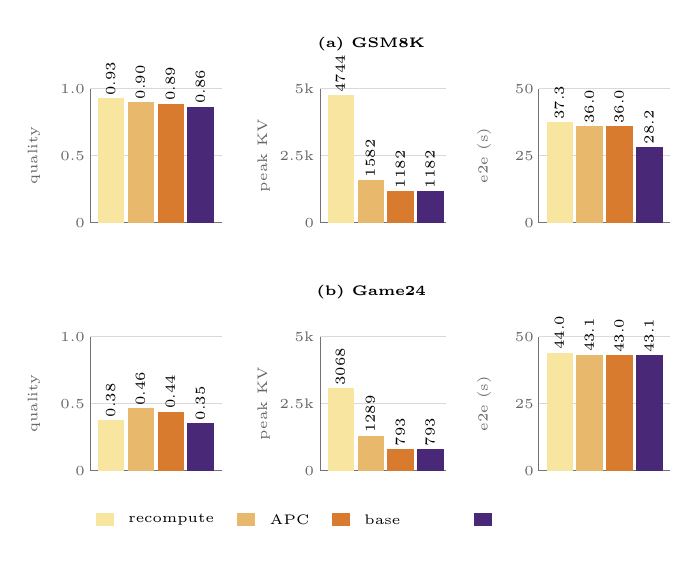
\begin{tikzpicture}[
  font=\scriptsize\sffamily,
  bar/.style={draw=black!55, line width=0.2pt},
  ax/.style={black!55, line width=0.35pt},
  grid/.style={black!15, line width=0.25pt},
  tick/.style={font=\tiny, text=black!60, inner sep=0pt},
  val/.style={font=\tiny, inner sep=0.3pt},
]
\definecolor{Rec}{HTML}{F8E6A0}
\definecolor{APC}{HTML}{E8B86D}
\definecolor{FS}{HTML}{D97B2F}
\definecolor{FSp}{HTML}{4A2878}

% --- (a) GSM8K, y shift 3.15 ---
\begin{scope}[shift={(0,3.15)}]
  \node[font=\tiny\bfseries] at (4.05,2.55) {(a) GSM8K};
  % quality, ymax 1.0
  \begin{scope}[shift={(0,0)}]
    \draw[grid] (0.48,0.28) -- (2.15,0.28) (0.48,1.13) -- (2.15,1.13) (0.48,1.98) -- (2.15,1.98);
    \draw[ax] (0.48,0.28) -- (2.15,0.28) (0.48,0.28) -- (0.48,1.98);
    \node[tick, anchor=east] at (0.42,0.28) {0};
    \node[tick, anchor=east] at (0.42,1.13) {0.5};
    \node[tick, anchor=east] at (0.42,1.98) {1.0};
    \node[tick, rotate=90, anchor=south] at (-0.15,1.13) {quality};
    \fill[bar, Rec] (0.58,0.28) rectangle (0.90,1.853);
    \fill[bar, APC] (0.96,0.28) rectangle (1.28,1.810);
    \fill[bar, FS]  (1.34,0.28) rectangle (1.66,1.788);
    \fill[bar, FSp] (1.72,0.28) rectangle (2.04,1.747);
    \node[val, rotate=90, anchor=west] at (0.74,1.87) {0.93};
    \node[val, rotate=90, anchor=west] at (1.12,1.83) {0.90};
    \node[val, rotate=90, anchor=west] at (1.50,1.81) {0.89};
    \node[val, rotate=90, anchor=west] at (1.88,1.77) {0.86};
  \end{scope}
  % peak KV, ymax 5k
  \begin{scope}[shift={(2.85,0)}]
    \draw[grid] (0.55,0.28) -- (2.15,0.28) (0.55,1.13) -- (2.15,1.13) (0.55,1.98) -- (2.15,1.98);
    \draw[ax] (0.55,0.28) -- (2.15,0.28) (0.55,0.28) -- (0.55,1.98);
    \node[tick, anchor=east] at (0.48,0.28) {0};
    \node[tick, anchor=east] at (0.48,1.13) {2.5k};
    \node[tick, anchor=east] at (0.48,1.98) {5k};
    \node[tick, rotate=90, anchor=south] at (-0.08,1.13) {peak KV};
    \fill[bar, Rec] (0.65,0.28) rectangle (0.97,1.893);
    \fill[bar, APC] (1.03,0.28) rectangle (1.35,0.818);
    \fill[bar, FS]  (1.41,0.28) rectangle (1.73,0.682);
    \fill[bar, FSp] (1.79,0.28) rectangle (2.11,0.682);
    \node[val, rotate=90, anchor=west] at (0.81,1.91) {4744};
    \node[val, rotate=90, anchor=west] at (1.19,0.84) {1582};
    \node[val, rotate=90, anchor=west] at (1.57,0.70) {1182};
    \node[val, rotate=90, anchor=west] at (1.95,0.70) {1182};
  \end{scope}
  % e2e seconds, ymax 50, shorter is faster
  \begin{scope}[shift={(5.70,0)}]
    \draw[grid] (0.48,0.28) -- (2.15,0.28) (0.48,1.13) -- (2.15,1.13) (0.48,1.98) -- (2.15,1.98);
    \draw[ax] (0.48,0.28) -- (2.15,0.28) (0.48,0.28) -- (0.48,1.98);
    \node[tick, anchor=east] at (0.42,0.28) {0};
    \node[tick, anchor=east] at (0.42,1.13) {25};
    \node[tick, anchor=east] at (0.42,1.98) {50};
    \node[tick, rotate=90, anchor=south] at (-0.12,1.13) {e2e (s)};
    \fill[bar, Rec] (0.58,0.28) rectangle (0.90,1.550);
    \fill[bar, APC] (0.96,0.28) rectangle (1.28,1.504);
    \fill[bar, FS]  (1.34,0.28) rectangle (1.66,1.505);
    \fill[bar, FSp] (1.72,0.28) rectangle (2.04,1.239);
    \node[val, rotate=90, anchor=west] at (0.74,1.57) {37.3};
    \node[val, rotate=90, anchor=west] at (1.12,1.52) {36.0};
    \node[val, rotate=90, anchor=west] at (1.50,1.52) {36.0};
    \node[val, rotate=90, anchor=west] at (1.88,1.26) {28.2};
  \end{scope}
\end{scope}

% --- (b) Game24 ---
\begin{scope}[shift={(0,0)}]
  \node[font=\tiny\bfseries] at (4.05,2.55) {(b) Game24};
  \begin{scope}[shift={(0,0)}]
    \draw[grid] (0.48,0.28) -- (2.15,0.28) (0.48,1.13) -- (2.15,1.13) (0.48,1.98) -- (2.15,1.98);
    \draw[ax] (0.48,0.28) -- (2.15,0.28) (0.48,0.28) -- (0.48,1.98);
    \node[tick, anchor=east] at (0.42,0.28) {0};
    \node[tick, anchor=east] at (0.42,1.13) {0.5};
    \node[tick, anchor=east] at (0.42,1.98) {1.0};
    \node[tick, rotate=90, anchor=south] at (-0.15,1.13) {quality};
    \fill[bar, Rec] (0.58,0.28) rectangle (0.90,0.917);
    \fill[bar, APC] (0.96,0.28) rectangle (1.28,1.067);
    \fill[bar, FS]  (1.34,0.28) rectangle (1.66,1.025);
    \fill[bar, FSp] (1.72,0.28) rectangle (2.04,0.875);
    \node[val, rotate=90, anchor=west] at (0.74,0.94) {0.38};
    \node[val, rotate=90, anchor=west] at (1.12,1.09) {0.46};
    \node[val, rotate=90, anchor=west] at (1.50,1.05) {0.44};
    \node[val, rotate=90, anchor=west] at (1.88,0.90) {0.35};
  \end{scope}
  \begin{scope}[shift={(2.85,0)}]
    \draw[grid] (0.55,0.28) -- (2.15,0.28) (0.55,1.13) -- (2.15,1.13) (0.55,1.98) -- (2.15,1.98);
    \draw[ax] (0.55,0.28) -- (2.15,0.28) (0.55,0.28) -- (0.55,1.98);
    \node[tick, anchor=east] at (0.48,0.28) {0};
    \node[tick, anchor=east] at (0.48,1.13) {2.5k};
    \node[tick, anchor=east] at (0.48,1.98) {5k};
    \node[tick, rotate=90, anchor=south] at (-0.08,1.13) {peak KV};
    \fill[bar, Rec] (0.65,0.28) rectangle (0.97,1.323);
    \fill[bar, APC] (1.03,0.28) rectangle (1.35,0.718);
    \fill[bar, FS]  (1.41,0.28) rectangle (1.73,0.550);
    \fill[bar, FSp] (1.79,0.28) rectangle (2.11,0.550);
    \node[val, rotate=90, anchor=west] at (0.81,1.34) {3068};
    \node[val, rotate=90, anchor=west] at (1.19,0.74) {1289};
    \node[val, rotate=90, anchor=west] at (1.57,0.57) {793};
    \node[val, rotate=90, anchor=west] at (1.95,0.57) {793};
  \end{scope}
  \begin{scope}[shift={(5.70,0)}]
    \draw[grid] (0.48,0.28) -- (2.15,0.28) (0.48,1.13) -- (2.15,1.13) (0.48,1.98) -- (2.15,1.98);
    \draw[ax] (0.48,0.28) -- (2.15,0.28) (0.48,0.28) -- (0.48,1.98);
    \node[tick, anchor=east] at (0.42,0.28) {0};
    \node[tick, anchor=east] at (0.42,1.13) {25};
    \node[tick, anchor=east] at (0.42,1.98) {50};
    \node[tick, rotate=90, anchor=south] at (-0.12,1.13) {e2e (s)};
    \fill[bar, Rec] (0.58,0.28) rectangle (0.90,1.775);
    \fill[bar, APC] (0.96,0.28) rectangle (1.28,1.747);
    \fill[bar, FS]  (1.34,0.28) rectangle (1.66,1.741);
    \fill[bar, FSp] (1.72,0.28) rectangle (2.04,1.744);
    \node[val, rotate=90, anchor=west] at (0.74,1.80) {44.0};
    \node[val, rotate=90, anchor=west] at (1.12,1.77) {43.1};
    \node[val, rotate=90, anchor=west] at (1.50,1.76) {43.0};
    \node[val, rotate=90, anchor=west] at (1.88,1.76) {43.1};
  \end{scope}
\end{scope}

\fill[Rec] (0.55,-0.42) rectangle (0.78,-0.26);
\node[font=\tiny, anchor=west] at (0.84,-0.34) {recompute};
\fill[APC] (2.35,-0.42) rectangle (2.58,-0.26);
\node[font=\tiny, anchor=west] at (2.64,-0.34) {APC};
\fill[FS] (3.55,-0.42) rectangle (3.78,-0.26);
\node[font=\tiny, anchor=west] at (3.84,-0.34) {base};
\fill[FSp] (5.35,-0.42) rectangle (5.58,-0.26);
\node[font=\tiny, anchor=west] at (5.64,-0.34) {\sys};
\end{tikzpicture}
}
\caption{Four systems on Qwen3-8B ($n{=}80$, $\mathrm{tp}{=}2$, $D{=}512$).
Each panel has its own axis.
Quality is higher-better; peak KV and end-to-end time are measured values, so a shorter bar is better.
(a)~GSM8K. (b)~Game24.
\sys lowers peak KV below APC on both workloads.
GSM8K quality stays with APC, and \sys also lowers GSM8K end-to-end time.}
\label{fig:eval-radar}
\end{figure*}

\begin{figure}[t]
\centering
\resizebox{\columnwidth}{!}{\begin{tikzpicture}[
  font=\scriptsize\sffamily,
  >=Latex,
  tick/.style={font=\tiny, text=black!55, inner sep=0pt},
  grid/.style={black!12, line width=0.25pt},
]
\definecolor{APC}{HTML}{C48A3A}
\definecolor{FSln}{HTML}{D97B2F}

% Measured DeepSeek-R1 GSM8K peaks: APC 761 tok, spine 561 tok.
% 8 GiB pool, 147456 B/token -> C = 76 and 103.
% Service model: e2e = 0.4 s, 256 decode tokens, so one slot is 640 tok/s.
% tok/s = min(round(qps*0.4), C) * 640.
% qps:     8, 32, 64, 128, 192, 256, 320, 384, 448, 512
% APC:  1920, 8320, 16640, 32640, 48640, then 48640
% FS:   1920, 8320, 16640, 32640, 49280, 65280, then 65920
% P99 s, APC: 0.020 until 128, 0.031, 0.294, 0.567, 0.841, 1.104, 1.378
% P99 s, FS:  0.020 until 256, 0.214, 0.416, 0.610, 0.812
% Left y: thousands, 0--80.  x: 512 * 0.0066 = 3.38

\begin{scope}[shift={(0,0)}]
  \foreach \y in {0,20,40,60,80} {
    \draw[grid] (0,\y*0.032) -- (3.55,\y*0.032);
    \node[tick, anchor=east] at (-0.06,\y*0.032) {\y};
  }
  \draw[black!55, line width=0.35pt] (0,0) -- (3.55,0);
  \draw[black!55, line width=0.35pt] (0,0) -- (0,2.56);
  % APC plateau 48.64, spine plateau 65.92
  \draw[APC, densely dashed, line width=0.3pt] (0,48.64*0.032) -- (3.55,48.64*0.032);
  \draw[FSln, densely dashed, line width=0.3pt] (0,65.92*0.032) -- (3.55,65.92*0.032);
  \draw[APC, line width=0.8pt]
    (8*0.0066, 1.92*0.032) -- (32*0.0066, 8.32*0.032) -- (64*0.0066, 16.64*0.032)
    -- (128*0.0066, 32.64*0.032) -- (192*0.0066, 48.64*0.032) -- (512*0.0066, 48.64*0.032);
  \draw[FSln, line width=0.8pt]
    (8*0.0066, 1.92*0.032) -- (32*0.0066, 8.32*0.032) -- (64*0.0066, 16.64*0.032)
    -- (128*0.0066, 32.64*0.032) -- (192*0.0066, 49.28*0.032) -- (256*0.0066, 65.28*0.032)
    -- (320*0.0066, 65.92*0.032) -- (512*0.0066, 65.92*0.032);
  \foreach \q/\ya/\yf in {8/1.92/1.92, 128/32.64/32.64, 192/48.64/49.28, 256/48.64/65.28, 512/48.64/65.92} {
    \fill[APC] (\q*0.0066, \ya*0.032) circle (1.15pt);
    \fill[FSln] (\q*0.0066, \yf*0.032) circle (1.15pt);
  }
  \draw[fsgain, line width=0.4pt] (3.28,48.64*0.032) -- (3.28,65.92*0.032);
  \node[font=\tiny, text=fsgain, anchor=east] at (3.20,1.83) {$+35.5\%$};
  \foreach \q/\lab in {8/8, 128/128, 256/256, 384/384, 512/512} {
    \node[tick] at (\q*0.0066, -0.18) {\lab};
  }
  \node[font=\tiny, anchor=south] at (1.78,2.62) {tok/s ($\times 10^{3}$)};
  \node[tick] at (1.78, -0.42) {offered QPS};
\end{scope}

\begin{scope}[shift={(4.55,0)}]
  \foreach \y in {0.0,0.5,1.0,1.5} {
    \draw[grid] (0,\y*1.60) -- (3.55,\y*1.60);
    \node[tick, anchor=east] at (-0.06,\y*1.60) {\y};
  }
  \draw[black!55, line width=0.35pt] (0,0) -- (3.55,0);
  \draw[black!55, line width=0.35pt] (0,0) -- (0,2.56);
  \draw[black!45, densely dashed] (0,1.60) -- (3.55,1.60);
  \node[tick, anchor=west, text=black!50] at (0.08,1.72) {SLO $1$\,s};
  \draw[APC, line width=0.8pt]
    (8*0.0066, 0.020*1.60) -- (128*0.0066, 0.020*1.60) -- (192*0.0066, 0.031*1.60)
    -- (256*0.0066, 0.294*1.60) -- (320*0.0066, 0.567*1.60) -- (384*0.0066, 0.841*1.60)
    -- (448*0.0066, 1.104*1.60) -- (512*0.0066, 1.378*1.60);
  \draw[FSln, line width=0.8pt]
    (8*0.0066, 0.020*1.60) -- (256*0.0066, 0.020*1.60) -- (320*0.0066, 0.214*1.60)
    -- (384*0.0066, 0.416*1.60) -- (448*0.0066, 0.610*1.60) -- (512*0.0066, 0.812*1.60);
  \fill[APC] (384*0.0066, 0.841*1.60) circle (1.15pt);
  \fill[APC] (448*0.0066, 1.104*1.60) circle (1.15pt);
  \fill[FSln] (512*0.0066, 0.812*1.60) circle (1.15pt);
  \foreach \q/\lab in {8/8, 128/128, 256/256, 384/384, 512/512} {
    \node[tick] at (\q*0.0066, -0.18) {\lab};
  }
  \node[font=\tiny, anchor=south] at (1.78,2.62) {P99 TTFT (s)};
  \node[tick] at (1.78, -0.42) {offered QPS};
\end{scope}

\fill[APC] (2.15,-0.78) rectangle (2.40,-0.64);
\node[font=\tiny, anchor=west] at (2.46,-0.71) {APC};
\fill[FSln] (3.55,-0.78) rectangle (3.80,-0.64);
\node[font=\tiny, anchor=west] at (3.86,-0.71) {\sys};
\end{tikzpicture}
}
\caption{Offered-load sweep from the measured DeepSeek-R1 GSM8K peaks.
Left: saturated tokens per second plateau at concurrency times the decode rate.
Right: APC crosses the $1$\,s P99 line first; \sys stays under it at a higher QPS.}
\label{fig:eval-slo}
\end{figure}

